\chapter{Background and Definitions}
\label{sec:Background}
% neural networks 
In this section, we go over the preliminarily concepts that help understand the contributions of this work. We start by looking at the family of methods to which Deep Convolutional Neural Networks belong, followed by a more detailed look at deep Convolutional neural networks in question by describing the main components of CNNs. 

\section{Deep Learning}
\label{sec:dl}
%Today, \textit{Artificial Intelligence(AI)} is a thriving field with many practical applications and active research topics. We look to intelligent software to automate routine labor, understand speech or images, make diagnoses in medicine and support basic scientific research. 
One of the central challenges of Artificial Intelligence (AI) is solving the tasks that are easy for people to perform but hard for them to describe formally -- problems that we solve intuitively, that feel automatic, like recognizing spoken words or faces in images. One approach to that challenge is to allow computers to learn from experience and understand the world in terms of a hierarchy of concepts, where each concept is defined in terms of its relation to simpler concepts. This hierarchy of concepts allows the computer to learn complex notions by building them out of simpler ones. If we draw a graph showing how these concepts are built on top of each other, it would be a deep graph with many layers. For this reason, we call this approach \textit{Deep Learning}\cite{Goodfellow-et-al-2016-Book}.

Modern deep learning provides a very powerful framework for specially for supervised learning. By adding more layers and more units within a layer, a deep network can represent functions of increasing complexity. Most tasks that consist of mapping an input vector to an output vector, and that are easy for a human-being to perform quickly, can be accomplished via deep learning, given sufficiently large models and datasets of labeled training examples. Other tasks that cannot be described as associating one vector to another, or that are difficult enough such that a person would require time to think and reflect in order to accomplish the task, remain beyond the scope of deep learning for now\cite{Goodfellow-et-al-2016-Book}.

In other words,  Deep Learning is a new area of Machine Learning (ML) research, which has been introduced with the objective of moving ML closer to one of its original goals: Artificial Intelligence. Deep Learning is about learning multiple levels of representation and abstraction that help to make sense of data such as images, sound and text\cite{tutorial2014lisa}.  

Various deep learning architectures involves Artificial Neural Networks (ANN). Networks such as \textit{deep neural networks}, \textit{deep convolutional neural networks},\textit{ deep belief networks} and \textit{recurrent neural networks} have been applied to fields like computer vision, automatic speech recognition or natural language processing where they have set the state-of-the-art in recent years, as reviewed by \citeauthor{bengio2009learning} in \cite{bengio2009learning, bengio2013deep}. 

Besides improving the accuracy on different pattern recognition problems, one of the fundamental goals of Deep Learning is to move machine learning towards the automatic discovery of multiple levels of representation, reducing the need for feature extractors developed by domain experts \cite{bengio2013deep}. This is especially important, as noted by \citeauthor{bengio2009learning} in \cite{bengio2009learning}, for domains where the features are hard to formalize, such as for object recognition and detection tasks.

In the task of object object detection, deep architectures have been widely used to achieve state-of-the-art results as in\cite{krizhevsky2009learning,krizhevsky2012imagenet}, where the top published results use Convolutional Neural Networks \cite{ciresan2012multi}. Among all deep learning techniques, we will apply deep convolutional neural networks to tackle a specific vision problem. However, prior to delving into deep CNN, we intend to allude the basic concept of Neural networks and deep NN briefly, in order to help understand the proposed method in this Master thesis.

\section{Artificial Neural Networks}

Artificial Neural Networks are mathematical models that use a collection of simple computational units, called Neurons, interlinked in a network. These models are used in a variety of pattern recognition tasks, such as speech recognition, object detection, identification of cancerous cells, among others \cite{hertz1991introduction}. Artificial Neural Networks date back to 1943, with work by McCulloch \cite{mcculloch1943logical}. The motivation for studying neural networks was the fact that the human brain was superior to a computer at many tasks, a statement that holds true even today for tasks such as recognizing objects and faces, in spite of the huge advances in the processing speed in modern computers.

The neuron is the basic unit on Artificial Neural Networks, and it is used to construct more powerful models. A typical set of equations to describe Neural Networks is provided in \cite{williams1986learning}, and is also listed below for completeness. A single neuron implements a mathematical function given its inputs, to provide an output, as described in equation ~\ref{eq:neuron} and illustrated in figure~\ref{fig:neuron}.

\begin{figure}[H]
	\centering
	{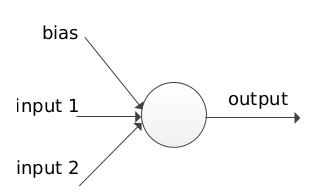
\includegraphics[width=0.45\textwidth]{images/neuron}}
	\caption{A single artificial neuron}
	\label{fig:neuron}
\end{figure}

\begin{equation}
f(x) = \sigma(\sum\limits_{i=1}^{n}x_iw_i + b) 
\label{eq:neuron}
\end{equation}

In this equation, $x_i$ is the input i, $w_i$ is the weight associated with input i, b is a bias term and $\sigma$ is a non-linear function. Common non-linear functions are Rectified Linear Unit non-linearity, and sigmoid function.

\subsection{Activation functions}
\label{sec:actfun}
To go from one layer to the next in a NN, units compute a weighted sum of their inputs from the previous layer and pass the result through a non-linear activation function\cite{lecun2015deep}. There are many possible choices for the non-linear activation functions in a multi-layered network, and the choice of activation functions for the hidden units may often be different from that for the output units. This is a consequence of the fact the hidden and output units perform different roles\cite{bishop1995neural}. 

\indent At present, the most popular non-linear function is the Rectified Linear Units (ReLU), which is simply the half-wave rectifier $f(z) = max(z, 0)$. In the past decades, neural nets used smoother non-linearities, such as $tanh(z)$ or $1/(1+ exp(-z))$, but ReLU typically learns much faster in networks with many layers, allowing training of a deep supervised network without unsupervised pre-training\cite{lecun2015deep}. A rectified linear unit has been illustrated in figure~\ref{fig:relu}

\begin{figure}[H]
	\centering
	{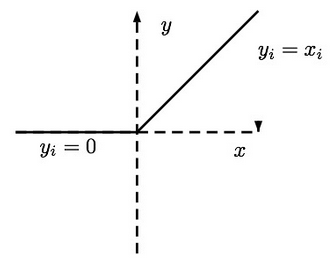
\includegraphics[width=0.4\textwidth]{images/relu}}
	\caption{A Rectified Linear Unit (ReLU)}
	\label{fig:relu}
\end{figure}

\indent The rectifier activation function allows a network to easily obtain sparse representations. For example, after uniform initialization of the weights, around 50\% of hidden units continuous output values are real zeros, and this fraction can easily increase with sparsity-including regularization. Apart from being more biologically plausible, sparsity also leads to mathematical advantages. On the other hand, one may hypothesize that the hard saturation at 0 may hurt optimization by blocking gradient back-propagation. However, experimental results done by\citeauthor{glorot2011deep} suggest that hard zeros can actually help supervised training\cite{glorot2011deep}.  


\subsection{Multi-layer Neural network}

Models based on a single neuron, also called Perceptrons, have severe limitations. As noted by \citeauthor{preparata2012computational}, a perceptron cannot model data that is not linearly separable, such as modeling a simple XOR operator. On the other hand, as shown by \citealt{hornik1989multilayer}, Multi-layer Neural Networks are universal approximators, that is: they can approximate any measurable function to any desired degree of accuracy.


A neural network of 3 or above layers of neurons shapes a \textit{Multi-layer Neural network} where the first layer is composed of the inputs to the neural network, it is followed by one or more \textit{hidden} layers, up to a last layer that contains the outputs of the network. In the simplest configuration, each layer l is fully connected with the adjacent layers $(l - 1 \& l + 1)$, and produces an output vector $y^{l}$ given the output vector of the previous layer y $^{l-1}$. The output of a layer is calculated by applying the neuron activation function for all neurons on the layer, as noted in equation ~\ref{eq:multi}, where $W^{l}$ is a matrix of weights assigned to each pair of neurons from layer \textit{l} and $l - 1$, and $b^{l}$ is a vector of bias terms for each neuron in layer \textit{l}.

\begin{equation}
y^{l} = \sigma(W^{l}y^{l-1}+ b^{l}) 
\label{eq:multi}
\end{equation}


\begin{figure}[H]
	\centering
	{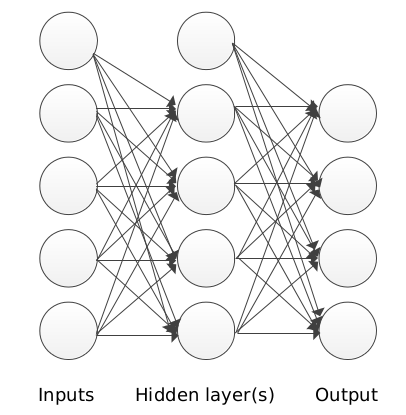
\includegraphics[width=0.45\textwidth]{images/mann}}
	\caption{A neural network composed of three layers}
	\label{fig:multi}
\end{figure}

\subsubsection{Training objective} 
In order to train the model, an error function, also called \textit{loss function}, is defined. This function calculates the error of the model predictions with respect to a dataset. The objective of the training is to minimize the sum (or, equivalently, minimize the mean) of this error function applied to all examples in the dataset. 

\indent Commonly used loss functions are the Squared Error function (SE), described in equation ~\ref{eq:SE}, and the Cross-Entropy error function (CE), described in equation ~\ref{eq:CE} (both equations describe the error for a single example in the dataset). As analyzed by \citealt{golik2013cross}, it can be shown that the true posterior probability is a global minimum for both functions, and therefore a Neural Network can be trained by minimizing either. 

\begin{equation}
E = \frac{1}{2} \sum\limits_{n} ( \hat{y_n}^{l} - y_n ){^2}
\label{eq:SE}
\end{equation}

\begin{equation}
E = -\sum\limits_{n}(y_n \log \hat{y_c}^{l})^{2}
\label{eq:CE}
\end{equation}

In these equations, $\hat{y_n}^{l}$ is the prediction of the model on the last layer for the unit \textit{c}, and $y_n$  is the corresponding true label.

For regression strategy, \textit{Euclidean loss} (Sum-of-Squares) function is commonly applied to the top of the outputs to compute Euclidean (L2)loss for real-valued regression tasks.
 


\subsubsection{Back Propagation}
\label{subsec:bp}

The error function can be minimized using Gradient-Based Learning. This strategy consists in taking partial derivatives of the error function with respect to the model parameters, and using these derivatives to iteratively update the parameters \cite{lecun1998gradient}. Efficient learning algorithms can be used for this purpose if these gradients (partial derivatives) can be computed analytically.

\textit{Backward Propagation} of errors (BP) was the main advance in the 1980's that led to an explosion of interest in NNs. BP is one of the most commonly used methods for training NNs. The idea behind BP is that it repeatedly adjusts the weights of the connections in the network so as to minimize a measure of the difference between the actual output vector of the network and the desired one. As a result of the weight adjustments, internal \textit{hidden} units come to represent important features of the task domain, and the regularities in the task are captured by the interactions of these units\cite{williams1986learning}.

Specifically, BP computes how fast the error changes as we adjust a hidden activity by using error derivatives with respect to hidden activities. Since each hidden activity can have a notable effect on many output units and consequently on the error, a combination of these effects must be considered. This aggregation is done efficiently which allows us to compute error derivatives for all the hidden units quickly at the same time. 

\indent Computing the error derivatives for the hidden activities, it would be easy to get the error derivatives for the weights going into a hidden unit which is the key to be able to learn efficiently. 
%For the first-layer weights, $w_{hj}$ , we use the chain rule to calculate the gradient, as described in \cite{alpaydin2014introduction}:
%
%\begin{equation}
%\frac{\delta E}{\delta w_{hj}} = \frac{\delta E}{\delta y_i} \frac{\delta y_i}{\delta z_h} \frac{\delta z_h}{\delta w_{hj}}
%\label{eq:CE}
%\end{equation}
%\indent Where $y_i$ is the output of the neuron, $z_h$ is the output before applying the activation function, and $w_{hj}$ ’s are the weights. It is as if the error propagates from the output y back to the inputs.
%
\section{Deep Neural Networks}
\label{sec:deepcnn}
As mentioned, standard neural network (NN) consists of many simple neurons, each producing a sequence of real-valued activations\cite{deepnn}. The depth of an architecture refers to the number of non-linear operations that are composed on the network. While many of the early successful applications of neural networks used shallow architectures (up to 3 levels), the mammal brain is organized in a deep architecture. The brain appears to process information through multiple stages, which is particularly clear in the primate visual system \cite{bengio2009learning}.

Moreover, theoretical results strongly suggest that in order to learn the kind of complicated functions that can represent high-level abstractions (e.g. in vision, language, and other AI-level tasks), one needs deep architectures. Deep Neural Networks are composed of multiple levels of non-linear operations, such as those present in neural nets with many hidden layers\cite{bengio2009learning}. figure~\ref{fig:deepl} demonstrates a deep neural network. 

\begin{figure}[H]
	\centering
	{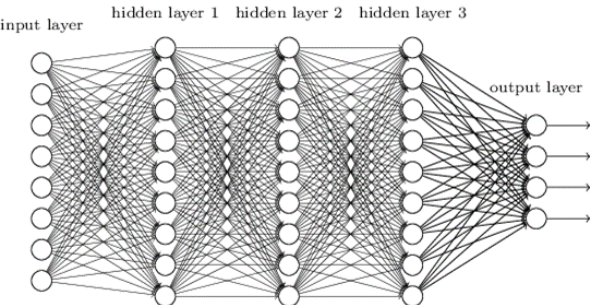
\includegraphics[width=0.7\textwidth]{images/deepnn}}
	\caption{A deep neural network with three hidden layers}
	\label{fig:deepl}
\end{figure}

Deep Neural Networks have been investigated for decades, but training deep networks consistently yielded poor results, until very recently. It was observed in many experiments that deep networks are harder to train than shallow networks, and that training deep networks often get stuck in apparent local minima (or plateaus) when starting with random initialization of the network parameters.

It was discovered, however, that better results could be achieved by pre-training each layer with an unsupervised learning algorithm \cite{hinton2006fast}. In 2006, \citeauthor{hinton2006fast} obtained good results using Restricted Boltzmann Machines (a generative model) to perform unsupervised training of the layers \cite{hinton2006fast}. The goal of this training was to obtain a model that could capture patterns in the data, similarly to a feature descriptor, not using the dataset labels. The weights learned by this unsupervised training were then used to initialize neural networks. 

\indent Similar results were reported using auto-encoders for training each layer \cite{bengio2007greedy}. These experiments identified that layers could be pre-trained one at a time, in a greedy layer-wise format. After the layers are pre-trained, the learned weights are used to initialize the neural network, and then the standard back-propagation algorithm (explained in ~\ref{subsec:bp}) is used for fine-tuning the network. The advantage of unsupervised pre-training was demonstrated in several statistical comparisons \cite{bengio2007greedy,larochelle2007empirical,erhan2009difficulty}, until recently, when deep neural networks trained only with supervised learning started to register similar results in some tasks (like object recognition). \citealt{ciresan2012multi} demonstrate that properly trained deep neural networks (with only supervised learning) are able to achieve top results in many tasks, although not denying that pre-training might help, especially in cases were little data is available for training, or when there are massive amounts of unlabeled data. On the task of image classification, the best published results use a particular type of architecture called Convolutional Neural Network, which is described ~\ref{sec:cnn}.



\section{Convolutional Neural Networks}
\label{sec:cnn}
Convolutional Neural Networks are a specialized kind of neural network for processing data that has a known grid-like topology such as image data which can be thought of as a 2D grid of pixels. CNN are simply neural networks that use convolution in place of general matrix multiplication in at least one of their layers \cite{Goodfellow-et-al-2016-Book}. This type of network was used to obtain state-of-the-art results in the CIFAR-10 object recognition task \cite{ciresan2012multi} and, more recently, to obtain state-of-the-art results in more challenging tasks such as the ImageNet Large Scale Visual Recognition Challenge \cite{russakovsky2015imagenet}. For both tasks, the training process benefited from the significant speed-ups on processing using modern GPUs (Graphical Processing Units), which are well suited for the implementation of convolutional networks.


Essentially, CNNs combine three architectural ideas to ensure some degree of shift and distortion invariance of local receptive fields, shared weights (or weight replication), and, sometimes, spatial or temporal sub-sampling\cite{lecun2010convolutional}. we are going to explain these basic ideas of CNN while introducing the main components that compose the main body of any CNN architecture.

\subsection{Convolutional layer} 
\label{convlayer}
Each unit of a convolutional layer receives inputs from a set of units located in a small neighborhood in the previous layer. With local receptive fields, neurons can extract elementary visual features such as oriented edges, end-points and corners. These features are then combined by the higher layers\cite{lecun2010convolutional}. In addition, elementary feature detectors that are useful on one part of the image are likely to be useful across the entire image. This knowledge can be applied by forcing a set of units, whose receptive fields are located at different places on the image, to have identical weight vectors\cite{williams1986learning}. The outputs of such a set of neurons constitutes a \textit{feature map}. At each position, different types of units in various feature maps compute distinct types of features. Figure~\ref{fig:cnnsample} presents a convolutional layer functionality during forward propagation. 

\begin{figure}[H]
	\centering
	{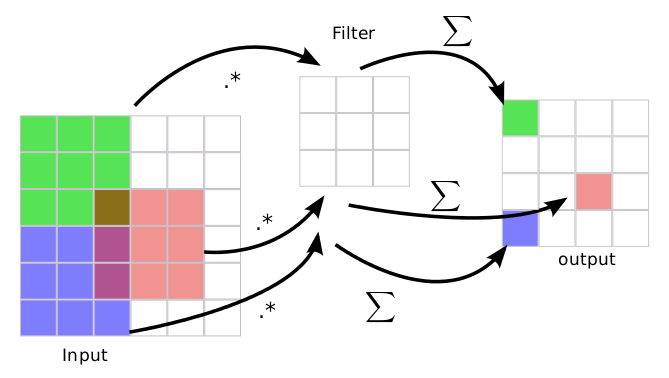
\includegraphics[width=0.7\textwidth]{images/conv}}
	\caption{The forward propagation phase of a convolutional layer}
	\label{fig:cnnsample}
\end{figure}
 
A sequential implementation of this process, for each feature map, would be to scan the input image with a single neuron that has a local receptive field, and to store the states of this neuron at corresponding locations in the feature map\cite{lecun2010convolutional}. \\
\indent Units in a feature map are constrained to perform the same operation on different parts ot the image. A convolutional layer is usually composed of several feature maps (with different weight vectors), so that multiple features can be extracted at each location. 

\noindent More formally, the definition of a 2D convolution is formulated in equation~\ref{eq:convf}. It is the
application of a discrete convolution of the inputs $y^{l-1}$ with a filter $w^{l}$ , adding a bias $b^{l}$, followed by the application of a non-linear function $\sigma$:

\begin{equation}
y_{rc}^{l} =  \sigma \sum_{i=1}^{F_r}\sum_{j=1}^{F_c}  y_{(r+i-1)(c+j-1)}^{l-1} w_{ij}^{l} + b^{l})
\label{eq:convf}
\end{equation}
l
In this equation, $y_{rc}^{l}$ is the output unit at \{r, c\}, $F_r$ and $F_c$ are the number of rows and columns in the 2D filter, $w_{ij}^{l}$ is the value of the filter at position \{i, j\},  $y_{(r+i-1)(c+j-1)}^{l-1}$ is the value of input to this layer, at position \{r + i - 1, c + j - 1\}, and $b^{l}$ is the bias term.

The equation above is defined for all possible applications of the filter, that is, for r $\in$ \{1, ..., $X_r$ - $F_r$ + 1\} and c $\in$ \{1, ..., $X_c$ - $F_c$ + 1\}, where $X_r$ and $X_c$ are the number of rows and columns in the input to this layer. The convolutional layer can either apply the filters for all possible inputs, or use a different strategy. Mainly to reduce computation time, instead of applying the filter for all possible \{r, c\} pairs, only the pairs with distances are used, which is called the \textit{stride}. A stride, s = 1, is equivalent to apply the convolution for all possible pairs, as defined above. 

\noindent The inspiration for convolutional layers originated from models of the mammal visual system. Modern research in the physiology of the visual system found it consistent with the processing mechanism of convolutional neural networks, at least for quick recognition of objects \cite{bengio2009learning}. Although being a biological plausible model, the theoretical reasons for the success of convolutional networks are not yet fully understood. One hypothesis is that the small fan-in of the neurons (i.e. the number or input connections to the neurons) helps the derivatives to propagate through many layers - instead of being diffused in a large number of input neurons.

\subsubsection{Weight Sharing}

Weight sharing refers to having several connections controlled by a single parameter (weight). Weight sharing can be interpreted as imposing equality constraints among the connection strengths. An interesting feature of weight sharing is that it can be implemented with very little computational overhead\cite{lecun1989generalization}. The weight sharing technique has an interesting side effect of reducing the number of free parameters, thereby the capacity of the machine and improving its generalization ability\cite{lecun2010convolutional}.



\subsection{Pooling/Sub-sampling layer}
\label{poolinglayer}
Once a feature is detected, its' exact position becomes less important as long as its' approximate position relative to other features is preserved. Furthermore, as the dimensionality of applying a filter is equal to the input dimensionality, we would not be gaining any translation invariance with these additional filters, we would be stuck doing pixel-wise analysis on increasingly abstract features. In order to solve this problem, a \textit{sub-sampling} layer is introduced.

 Sub-sampling, or down-sampling, refers to reducing the overall size of a signal. In many cases, such as audio compression for music files, sub-sampling is done simply for size reduction \cite{sub}. But in the domain of 2D filter outputs, sub-sampling  can also be thought of as reducing the sensitivity of the output to shifts and distortions.

One of the most applied sub-sampling methods used in \cite{lecun1995comparison}, is known as \textit{max-pooling}. Equation ~\ref{eq:pool} presents te formulation of a max-pooling layer. 

\begin{equation}
y_{rc}^{l} =  \max_{i,j\in\{0,1,...,m\} }  y_{(r+i-1)(c+j-1)}^{l-1}
\label{eq:pool}
\end{equation}
In this equation, $y_{rc}^{l}$ is the output for index \textit{{r, c}}, \textit{m} is the size of the pooling area, and $y_{(r+i-1)(c+j-1)}^{l-1}$ is the value of the input at the position \{r + i - 1, c + j - 1\}.


 
This involves splitting up the matrix of filter outputs into small non-overlapping grids (the larger the grid, the greater the signal reduction), and taking the maximum value in each grid as the value in the reduced matrix. A schematic of max-pooling is depicted in figure~\ref{fig:pooling}.Similarly for the convolutional layer described above, instead of generating all possible pairs of \{i, j\}, a \textit{stride, s,} can be used. In particular, a stride s = 1 is equivalent to using all possible pooling windows, and a stride s = m is equivalent of using all non-overlapping pooling windows.
\begin{figure}[H]
	\centering
	{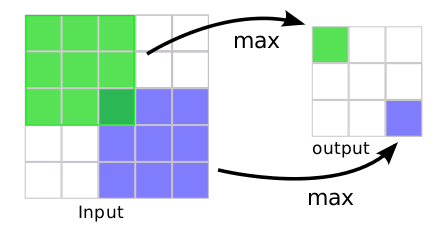
\includegraphics[width=0.5\textwidth]{images/pooling}}
	\caption{The forward propagation phase of a pooling layer with stride equal to 1.}
	\label{fig:pooling}
\end{figure}
 
\citealt{scherer2010evaluation} evaluated different pooling architectures, and note that the max-pooling layers obtained the best results. Pooling layers add robustness to the model, providing a small degree of translation invariance, since the unit activates independently on where the image feature is located within the pooling window \cite{bengio2013deep}. Empirically, pooling has demonstrated to contribute to improved classification accuracy for object recognition \cite{lecun1989backpropagation}.


\subsection{Local Response Normalization}
\label{lrnlayer}
ReLU have the desirable property that they do not require input normalization to prevent them from saturating. If at least some training examples produce a positive input to a ReLU, learning will happen in that neuron. However, we still find that \textit{local response normalization}(LRN) scheme aids generalization. This sort of response normalization implements a form of lateral inhibition ( the capacity of an excited neuron to reduce the activity of its neighbors) inspired by the type found in real neurons, creating competition for big activities amongst neuron outputs computed using different kernels\cite{krizhevsky2012imagenet}. 

In other words, we can think of it as helping sharpening the response. Instead of carrying multiple ambiguous representation of a patch, it pushes the network to commit more towards a specific representation, freeing resources to analyze it better.

\indent This scheme bears some resemblance to the local contrast normalization scheme proposed by \citeauthor{jarrett2009best} in \cite{jarrett2009best} which has led to error rate reduction in \cite{krizhevsky2012imagenet} and \cite{hinton2012improving}. 

\subsection{Fully connected/Inner product layer}

Finally, after several convolutional and max pooling layers, the high-level reasoning in the neural network is done via \textit{fully connected layers}(IP). A fully connected layer takes all neurons in the previous layer (be it fully connected, pooling, or convolutional) and connects it to every single neuron it has. Fully connected layers are not spatially located anymore (you can visualize them as one-dimensional), so there can be no convolutional layers after a fully connected layer. 




